\chapter{Introduction to Root Based Arabic System}

%\textarabic{\quranayah[1][1]}

\textit{Root meaning + Pattern meaning = Word meaning}
%\begin{chapquote}{}
%Root meaning + Pattern meaning = Word meaning
%\end{chapquote}

\section{Roots}
\begin{itemize}	    \setlength{\itemsep}{5pt}
	\item Most of the words in Arabic language are formed from basic letters called `roots' or \textarabic{جذور}
	\item These roots are morphed in to patterns (\textarabic{الأوزان}) to form different meaningful words
	\item Most of the words have three roots and some have four. Very few have five or six roots also \\
	\textarabic{علم، خلق، عمل، ترك، كفر} are examples of 3 letter root \\
	\textarabic{وسوس، زلزل، ترجم} are examples of 4 letter root
	
	\item  If a root consists of two of the same letter right next to one another, it will often be represented as one letter with a \textarabic{sukuun} as in\\
		\textarabic{ح-ب-ب} \qquad \textarabic{حبّ} \qquad love
	
	\item We will add Prefixes, Suffixes and
	Infixes to Root to form additional
	words \\
	
	Prefix - something added at the beginning. \textbf{Eg:-}
	\underline{Un}lawful (lawful) , \underline{a}political (political) \\
	Suffix - something added at the end. \textbf{Eg:-}
	Invent\underline{ion} (invent) , place\underline{ment} 	(place) \\
	Infix - something added in 	between the word. 
	They are not used in English but are very common in Arabic
	
	
%	 \textarabic{علم} means he knew
	 

	
	
	\item Determining “Root” word is also helpful
	in finding its meaning in the dictionary \\
	For example, consider the word \textarabic{معلوم}, You won’t find its meaning under \textarabic{م} \\
	First find out the Root of \textarabic{معلوم} It is \textarabic{علم}
	Then look under \textarabic{ع} you will find \textarabic{معلوم}
	
	
\end{itemize}
Examples
\footnote{\url{https://studioarabiya.com/blog/learning-arabic/appreciating-arabic-three-letter-roots-1}}
\begin{itemize}	    \setlength{\itemsep}{5pt}
	\item The words \textarabic{Islam}, \textarabic{Muslim} (one who follows the religion of Islam), salaam (peace), \textarabic{tasleem} (submission), \textarabic{silm} (peace treaty), and \textarabic{salamah} (well-being and wholeness) all come from the same three-letter root (\textarabic{س ل م})
	
	\item The word for a mother’s womb (\textarabic{رحم} rahim) is connected to the word for loving mercy (\textarabic{رحمة} rahma).
	
	\item  The word for beauty and perfection (\textarabic{إحسان} ihsan) is connected to the word for a good deed, and the reward of a goodly deed (\textarabic{حسنة} hasana).
	
%	\item  The word for a righteous person (\textarabic{صالح} salih) is related to words that mean to make amends, to rebuild or reconstruct, to bring together and to be a peacemaker.
\end{itemize}

Some of the words derived from \textarabic{ك-ت-ب}
\footnote{\url{https://www.softschools.com/languages/arabic/roots_and_patterns/}}
\begin{itemize}	    \setlength{\itemsep}{5pt}
	\item \textarabic{كِتاب} - a book
	\item \textarabic{كاتِب} - a writer
	\item \textarabic{مَكْتَب} - an office
	\item \textarabic{مَكْتَبة} - a library
	\item \textarabic{مَكْتوب} - a letter
	\item \textarabic{يَكْتَب} - he writes
	\item \textarabic{كَتَبَ} - he wrote
\end{itemize}
\section{Patterns}

\begin{itemize}	    \setlength{\itemsep}{5pt}
	\item Patterns are the set molds of words that roots can be inserted into. Together, the root letters placed inside the patterns are words. Patterns also carry meanings, similar to how suffixes and prefixes do so.
	\item The root \textarabic{ف-ع-ل} , meaning "to do," is often used to model patterns and will be used here to do so. In these contexts, \textarabic{ف-ع-ل} represents where you will insert the letters of any root into the pattern to create the full meaning. The first letter goes where \textarabic{ف} goes, the second where \textarabic{ع} goes and the third where \textarabic{ل} goes.
	
\end{itemize}




\section{Root based dictionaries}

%\selectlanguage{arabic}
Some of the root-based dictionaries are
\begin{enumerate}	    %\setlength{\itemsep}{5pt}
	\item \textarabic{كتاب العين}
	\item \textarabic{المعجم الوسيط}
	\item Hans Wehr
	\item Lame's Lexicon
\end{enumerate}

\noindent Some of `alif-ba-tical' dictionaries are
\begin{enumerate}	    %\setlength{\itemsep}{5pt}
	\item \textarabic{المورد}
%	\item \textarabic{المعجم الوسيط}
%	\item Hans Wehr
%	\item Lame's Lexicon
\end{enumerate}

\section{Why use a root-based dictionary}
\subsection{Vocab}
Many words are derived from a root. 
All the words derive from a root are given together in a root based dictionary. This will help the reader to understand their connection and hence to achieve greater vocabulary. 
Example: There are at least 31 words are derived from \textarabic{س ك ن}  \\

This is not the case in an `alif-ba-tical' dictionary where words are organized in the ascending order.
For example, the word  \textarabic{كَتَبَ} - (he wrote) - comes in the 7 pages after the  the word 	 \textarabic{كاتِب} - (a writer)-  in \textarabic{Al-mawrid}, an `alif-ba-tical' dictionary. This will not give any clue of their connection to the reader
%\begin{figure} 
%	\centering
%	\includegraphics[width=0.7\linewidth]{./images/almawridkataba}
%	\caption{}
%	\label{fig:almawridkataba}
%\end{figure}



\subsection{Roots are powerful}


\subsubsection{Guess the meaning of Words}
Understanding the meaning of a root and pattern in general will help to guess the meaning of any give word by identifying its root and pattern.\\


Root meaning + Pattern meaning = Word meaning \\

\begin{minipage}{.33\textwidth}
	\textarabic{الاستنساخ}
\end{minipage}
\begin{minipage}{.33\textwidth}
	\textarabic{ن س خ} \\ copying
\end{minipage}
\begin{minipage}{.33\textwidth}
	to clone
\end{minipage}

\subsubsection{Distinguish between synonyms}
No two words are exactly equivalent even they have listed as synonyms.
Understanding the root of synonyms will help to distinguish between them by understanding the what specific flavour is associated with it. \\ 

\begin{minipage}{.33\textwidth}
	word = \\ meaning = \\ root meaning =
\end{minipage}
\begin{minipage}{.33\textwidth}
	\textarabic{الغني} \\ wealthy \\ ``free from need"
\end{minipage}
\begin{minipage}{.33\textwidth}
	\textarabic{الثري} \\ wealthy \\ ``plenitude"
\end{minipage}
	
\subsubsection{Appreciate the Arab's \textit{Weltanschauung}}
Consider the example below, Both the words morph from the roots 
\textarabic{ع-ق-ل}
which generally means ``\textarabic{to-bind}". \\


\begin{minipage}{.33\textwidth}
	word = \\ meaning = \\ description =
\end{minipage} 
\begin{minipage}{.33\textwidth}
	\textarabic{عَقْلٌ} \\ intellect \\ binding a person to live
\end{minipage}
\begin{minipage}{.33\textwidth}
	\textarabic{عِقال} \\ hobbling cord \\ binding the animal
\end{minipage}

%
%\begin{minipage}{.33\textwidth}
%	\textarabic{كريم} \\ noble generous
%\end{minipage}


\section{Introduction to Hans Wehr}
\subsection{The best root-based dictionary}
\begin{itemize}	    \setlength{\itemsep}{5pt}
	\item Best organizing by root
	\item Prepositional usage without peer
	\item Modern usage	
\end{itemize}
\noindent Authored by, \\
Hans Wehr, Professor at University of Munster until 1974 \\
J. Milton Cowan, Professor at Cornell, President of Linguistic Society of America

\section{How to use Hans Wehr}
\subsection{Organization by roots}
\subsubsection{Organization of entries}
\begin{figure}
	\centering
	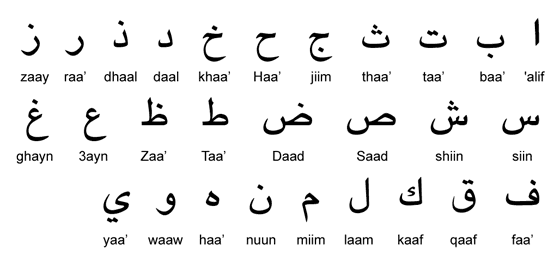
\includegraphics[width=0.7\linewidth]{chapters/images/alphabets}
	\caption{Arabic letters in alif-batical order}
	\label{fig:alphabets}
\end{figure}


\begin{itemize}	    \setlength{\itemsep}{5pt}
	\item Arabic words are organized by roots
	\item Foreign words are alif-batically placed 
\end{itemize}

\begin{figure}
\begin{minipage}{.5\textwidth}

		For Example, All the words originating from the roots \textarabic{مرغ} are placed together. \\
		
		The root \textarabic{مرق} comes after the root \textarabic{مرغ} as the letter \textarabic{ق} is alif-batically after the letter \textarabic{غ} \\
		
		The foreign words for \textit{margin} and \textit{morphine} are placed alif-batically with roots

\end{minipage}
\begin{minipage}{.5\textwidth}
	\quad  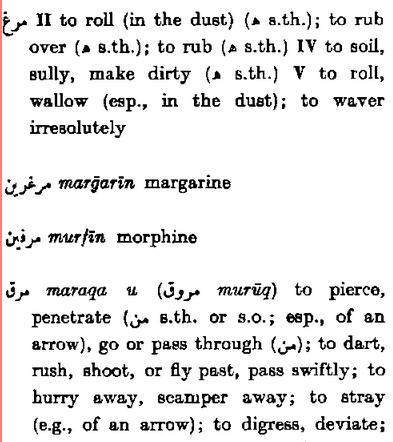
\includegraphics[width=.9\linewidth]{chapters/images/hans_mrg}
		\caption{The roots \textarabic{مرغ} and \textarabic{مرق} in HW}
\end{minipage}
\end{figure}

\begin{itemize}	    \setlength{\itemsep}{5pt}
	\item Words having weak letters needs special attention. \\ Weak letters \textarabic{(ا,و,ي)} are flexible. They may change with each other during the morphology \\
	For example, the words \textarabic{قال، قيل، قولو} are derived from the same root \textarabic{قول} \\
	When looking such words, you may have to look for all possibilities. \\ However, the letters \textarabic{ و\& ي } are generally the roots. \\
	When looking for the root of the word \textarabic{قال} one has to look at roots \textarabic{قول} and  \textarabic{قيل}. If found both, you will have to depend on the context of the word to ascertain. 

\begin{figure}[h]
	\begin{minipage}{.5\textwidth}

			\centering
			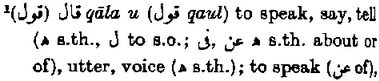
\includegraphics[width=0.95\linewidth]{chapters/images/qwl}
			\caption{Root \textarabic{قول}}
			\label{fig:qwl}

		
	\end{minipage}
	\begin{minipage}{.5\textwidth}
			\centering
		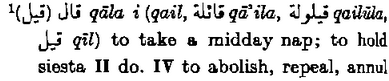
\includegraphics[width=0.95\linewidth]{chapters/images/qyl}
		\caption{Root \textarabic{قيل}}
		\label{fig:qyl}
		
	\end{minipage}
\end{figure}
	
	
	\item Doubled roots	\\ 
	Often, 2nd and 3rd root letters may come as the same as in \\
	\qquad word = \textarabic{قصّ} \qquad root = \textarabic{ق~ص~ص}  \qquad meaning = to cut \\
	
	In Hans Wehr, such roots are listed as if  there is no third letter. Hence, the root \textarabic{ق~ص~ص} is considered as \textarabic{ق ص} for listing. Here is the order of alif-batically nearer roots in the dictionary,
	
	\begin{itemize}	    \setlength{\itemsep}{5pt}
		\item \textarabic{ق ش ف}
		\item \textarabic{ق ص ص}
		\item \textarabic{ق ص ب}
		\item \textarabic{ق ص د}
	\end{itemize}
\end{itemize}



\subsection{Past tense options}
After the root letters given in Arabic, Hans gives the Form-I past tense transliterated in English. It follows the Arabic voweling as
\begin{itemize}	    \setlength{\itemsep}{5pt}
	\item a = fath-ha, \quad \textarabic{\_َ}
	\item i = kasra, \quad \textarabic{\_ِ}
	\item u = dhamma, \quad \textarabic{\_ُ}
	\item - = sukun,  \quad \textarabic{\_ْ}
%		\item un = dhamma thanveen,  \quad \textarabic{\_ٌ}
\end{itemize}

The same root can have multiple (Form-I) past tense options, changing the voweling and thus meaning. 
 

\begin{figure}[h]
	
	 \begin{minipage}{.5\textwidth}
		Consider the root \textarabic{ق د م}. It has 3 past tense options. 
		\begin{enumerate}	    \setlength{\itemsep}{5pt}
			\item \textarabic{قَدَمَ - يَقْدُمُ - قَدْمٌ، قُدُومٌ}
			\item \textarabic{قَدِمَ - يَقْدَمُ - قُدُومٌ، قِدْمَان، مَقْدَمٌ}
			\item \textarabic{قَدُمَ - يَقْدُمُ - قِدَمٌ}
		\end{enumerate}
	\end{minipage}
	 \begin{minipage}{.5\textwidth}
	 		\centering
	 		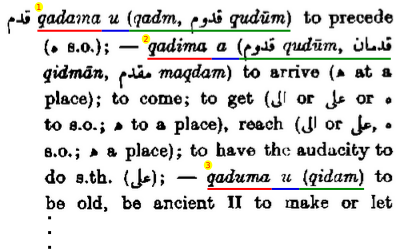
\includegraphics[width=0.9\linewidth]{./chapters/images/hansqdm}
	 		\caption{The listings under root \textarabic{ق د م}}
	 		\label{fig:hans-qdm}
	 \end{minipage}
\end{figure}
 
\subsection{Present tense options}
The Form-II present tense is of the form \textarabic{يَفْعَُِلُ} having properties,
\begin{itemize}	    %\setlength{\itemsep}{3pt}
	\item First is \textarabic{يَ} with fath-ha
	\item Second is the first letter of root with sukun
	\item Third is the second root letter which may carries fath-ha (a) or kasra (i) or dhamma (u). 
	\item Forth is the third root letter with dhamma. 
\end{itemize}

Hans gives the symbol on second root letter in the present tense (a, i or u) after the past tense option
\subsection{Verbal nouns} 
Verbal nouns \textarabic{المصدر} are given in parentheses after the past tense and present tense symbol in the transliterated form. 
\subsection{Prepositional usage}
\subsection{10 forms}
\subsection{Common phrases}
\subsection{Common nouns}


\section{Advanced way to use Hans Wehr}
\subsection{Checking translation for prediction}
\subsection{What to do if a word is not in Hans Wehr}
\section{Guided practice}


\section{Hans Wehr transliteration}
The Hans Wehr transliteration system is a system for transliteration of the Arabic alphabet into the Latin
alphabet used in the Hans Wehr dictionary (1952; in English 1961). The system was modified somewhat in the
English editions. It is printed in lowercase italics. It marks some consonants using diacritics (underdot, macron
below, and caron) rather than digraphs, and writes long vowels with macrons.
The transliteration of the Arabic alphabet:
\footnote{
	\url{https://en.wikipedia.org/wiki/Hans_Wehr_transliteration}}

\includepdf[pages={2,3}]{chapters/HansWehrtransliteration}

